% Options for packages loaded elsewhere
\PassOptionsToPackage{unicode}{hyperref}
\PassOptionsToPackage{hyphens}{url}
\PassOptionsToPackage{dvipsnames,svgnames,x11names}{xcolor}
%
\documentclass[
  letterpaper,
  DIV=11,
  numbers=noendperiod]{scrartcl}

\usepackage{amsmath,amssymb}
\usepackage{iftex}
\ifPDFTeX
  \usepackage[T1]{fontenc}
  \usepackage[utf8]{inputenc}
  \usepackage{textcomp} % provide euro and other symbols
\else % if luatex or xetex
  \usepackage{unicode-math}
  \defaultfontfeatures{Scale=MatchLowercase}
  \defaultfontfeatures[\rmfamily]{Ligatures=TeX,Scale=1}
\fi
\usepackage{lmodern}
\ifPDFTeX\else  
    % xetex/luatex font selection
\fi
% Use upquote if available, for straight quotes in verbatim environments
\IfFileExists{upquote.sty}{\usepackage{upquote}}{}
\IfFileExists{microtype.sty}{% use microtype if available
  \usepackage[]{microtype}
  \UseMicrotypeSet[protrusion]{basicmath} % disable protrusion for tt fonts
}{}
\makeatletter
\@ifundefined{KOMAClassName}{% if non-KOMA class
  \IfFileExists{parskip.sty}{%
    \usepackage{parskip}
  }{% else
    \setlength{\parindent}{0pt}
    \setlength{\parskip}{6pt plus 2pt minus 1pt}}
}{% if KOMA class
  \KOMAoptions{parskip=half}}
\makeatother
\usepackage{xcolor}
\setlength{\emergencystretch}{3em} % prevent overfull lines
\setcounter{secnumdepth}{4}
% Make \paragraph and \subparagraph free-standing
\makeatletter
\ifx\paragraph\undefined\else
  \let\oldparagraph\paragraph
  \renewcommand{\paragraph}{
    \@ifstar
      \xxxParagraphStar
      \xxxParagraphNoStar
  }
  \newcommand{\xxxParagraphStar}[1]{\oldparagraph*{#1}\mbox{}}
  \newcommand{\xxxParagraphNoStar}[1]{\oldparagraph{#1}\mbox{}}
\fi
\ifx\subparagraph\undefined\else
  \let\oldsubparagraph\subparagraph
  \renewcommand{\subparagraph}{
    \@ifstar
      \xxxSubParagraphStar
      \xxxSubParagraphNoStar
  }
  \newcommand{\xxxSubParagraphStar}[1]{\oldsubparagraph*{#1}\mbox{}}
  \newcommand{\xxxSubParagraphNoStar}[1]{\oldsubparagraph{#1}\mbox{}}
\fi
\makeatother

\usepackage{color}
\usepackage{fancyvrb}
\newcommand{\VerbBar}{|}
\newcommand{\VERB}{\Verb[commandchars=\\\{\}]}
\DefineVerbatimEnvironment{Highlighting}{Verbatim}{commandchars=\\\{\}}
% Add ',fontsize=\small' for more characters per line
\newenvironment{Shaded}{}{}
\newcommand{\AlertTok}[1]{\textcolor[rgb]{0.58,0.85,0.30}{\textbf{\colorbox[rgb]{0.30,0.12,0.14}{#1}}}}
\newcommand{\AnnotationTok}[1]{\textcolor[rgb]{0.31,0.63,0.31}{#1}}
\newcommand{\AttributeTok}[1]{\textcolor[rgb]{0.65,0.15,0.64}{#1}}
\newcommand{\BaseNTok}[1]{\textcolor[rgb]{0.60,0.41,0.00}{#1}}
\newcommand{\BuiltInTok}[1]{\textcolor[rgb]{0.65,0.15,0.64}{#1}}
\newcommand{\CharTok}[1]{\textcolor[rgb]{0.31,0.63,0.31}{#1}}
\newcommand{\CommentTok}[1]{\textcolor[rgb]{0.63,0.63,0.65}{\textit{#1}}}
\newcommand{\CommentVarTok}[1]{\textcolor[rgb]{0.89,0.34,0.29}{\textit{#1}}}
\newcommand{\ConstantTok}[1]{\textcolor[rgb]{0.60,0.41,0.00}{#1}}
\newcommand{\ControlFlowTok}[1]{\textcolor[rgb]{0.65,0.15,0.64}{#1}}
\newcommand{\DataTypeTok}[1]{\textcolor[rgb]{0.65,0.15,0.64}{#1}}
\newcommand{\DecValTok}[1]{\textcolor[rgb]{0.60,0.41,0.00}{#1}}
\newcommand{\DocumentationTok}[1]{\textcolor[rgb]{0.89,0.34,0.29}{#1}}
\newcommand{\ErrorTok}[1]{\textcolor[rgb]{0.96,0.28,0.28}{\underline{#1}}}
\newcommand{\ExtensionTok}[1]{\textcolor[rgb]{0.25,0.47,0.95}{\textbf{#1}}}
\newcommand{\FloatTok}[1]{\textcolor[rgb]{0.60,0.41,0.00}{#1}}
\newcommand{\FunctionTok}[1]{\textcolor[rgb]{0.25,0.47,0.95}{#1}}
\newcommand{\ImportTok}[1]{\textcolor[rgb]{0.31,0.63,0.31}{#1}}
\newcommand{\InformationTok}[1]{\textcolor[rgb]{0.77,0.36,0.00}{#1}}
\newcommand{\KeywordTok}[1]{\textcolor[rgb]{0.65,0.15,0.64}{#1}}
\newcommand{\NormalTok}[1]{\textcolor[rgb]{0.22,0.23,0.26}{#1}}
\newcommand{\OperatorTok}[1]{\textcolor[rgb]{0.65,0.15,0.64}{#1}}
\newcommand{\OtherTok}[1]{\textcolor[rgb]{0.15,0.68,0.38}{#1}}
\newcommand{\PreprocessorTok}[1]{\textcolor[rgb]{0.65,0.15,0.64}{#1}}
\newcommand{\RegionMarkerTok}[1]{\textcolor[rgb]{0.16,0.50,0.73}{\colorbox[rgb]{0.08,0.19,0.26}{#1}}}
\newcommand{\SpecialCharTok}[1]{\textcolor[rgb]{0.00,0.52,0.74}{#1}}
\newcommand{\SpecialStringTok}[1]{\textcolor[rgb]{0.85,0.27,0.33}{#1}}
\newcommand{\StringTok}[1]{\textcolor[rgb]{0.31,0.63,0.31}{#1}}
\newcommand{\VariableTok}[1]{\textcolor[rgb]{0.89,0.34,0.29}{#1}}
\newcommand{\VerbatimStringTok}[1]{\textcolor[rgb]{0.85,0.27,0.33}{#1}}
\newcommand{\WarningTok}[1]{\textcolor[rgb]{0.85,0.27,0.33}{#1}}

\providecommand{\tightlist}{%
  \setlength{\itemsep}{0pt}\setlength{\parskip}{0pt}}\usepackage{longtable,booktabs,array}
\usepackage{calc} % for calculating minipage widths
% Correct order of tables after \paragraph or \subparagraph
\usepackage{etoolbox}
\makeatletter
\patchcmd\longtable{\par}{\if@noskipsec\mbox{}\fi\par}{}{}
\makeatother
% Allow footnotes in longtable head/foot
\IfFileExists{footnotehyper.sty}{\usepackage{footnotehyper}}{\usepackage{footnote}}
\makesavenoteenv{longtable}
\usepackage{graphicx}
\makeatletter
\def\maxwidth{\ifdim\Gin@nat@width>\linewidth\linewidth\else\Gin@nat@width\fi}
\def\maxheight{\ifdim\Gin@nat@height>\textheight\textheight\else\Gin@nat@height\fi}
\makeatother
% Scale images if necessary, so that they will not overflow the page
% margins by default, and it is still possible to overwrite the defaults
% using explicit options in \includegraphics[width, height, ...]{}
\setkeys{Gin}{width=\maxwidth,height=\maxheight,keepaspectratio}
% Set default figure placement to htbp
\makeatletter
\def\fps@figure{htbp}
\makeatother

\usepackage{setspace}
\usepackage[most]{tcolorbox}

\newtcolorbox{note}{
	colback=gray!10,
	colframe=gray!80!black,
	boxrule=0.5pt,
	arc=2mm,
	left=6pt,
	right=6pt,
	top=6pt,
	bottom=6pt,
	enhanced,
	before upper={\setstretch{1.2}},
}

\newtcolorbox{example}{
	colback=blue!10,
	colframe=blue!80!black,
	boxrule=0.5pt,
	arc=2mm,
	left=6pt,
	right=6pt,
	top=6pt,
	bottom=6pt,
	enhanced,
	before upper={\setstretch{1.2}},
}

% \usepackage[most]{tcolorbox}
% \newtcolorbox{shadednote}{
%   colback=gray!10,
%   colframe=gray!80!black,
%   boxrule=0.5pt,
%   arc=2mm,
%   left=6pt,
%   right=6pt,
%   top=6pt,
%   bottom=6pt,
%   enhanced,
%   before upper=\relax, % Do nothing, let it inherit
% }
% \newtcolorbox{shadednote}{
%   colback=gray!10,
%   colframe=gray!80!black,
%   boxrule=0.5pt,
%   arc=2mm,
%   left=6pt,
%   right=6pt,
%   top=6pt,
%   bottom=6pt,
% }
\usepackage{booktabs}
\usepackage{longtable}
\usepackage{array}
\usepackage{multirow}
\usepackage{wrapfig}
\usepackage{float}
\usepackage{colortbl}
\usepackage{pdflscape}
\usepackage{tabu}
\usepackage{threeparttable}
\usepackage{threeparttablex}
\usepackage[normalem]{ulem}
\usepackage{makecell}
\usepackage{xcolor}
\KOMAoption{captions}{tableheading}
\makeatletter
\@ifpackageloaded{caption}{}{\usepackage{caption}}
\AtBeginDocument{%
\ifdefined\contentsname
  \renewcommand*\contentsname{Table of contents}
\else
  \newcommand\contentsname{Table of contents}
\fi
\ifdefined\listfigurename
  \renewcommand*\listfigurename{List of Figures}
\else
  \newcommand\listfigurename{List of Figures}
\fi
\ifdefined\listtablename
  \renewcommand*\listtablename{List of Tables}
\else
  \newcommand\listtablename{List of Tables}
\fi
\ifdefined\figurename
  \renewcommand*\figurename{Figure}
\else
  \newcommand\figurename{Figure}
\fi
\ifdefined\tablename
  \renewcommand*\tablename{Table}
\else
  \newcommand\tablename{Table}
\fi
}
\@ifpackageloaded{float}{}{\usepackage{float}}
\floatstyle{ruled}
\@ifundefined{c@chapter}{\newfloat{codelisting}{h}{lop}}{\newfloat{codelisting}{h}{lop}[chapter]}
\floatname{codelisting}{Listing}
\newcommand*\listoflistings{\listof{codelisting}{List of Listings}}
\makeatother
\makeatletter
\makeatother
\makeatletter
\@ifpackageloaded{caption}{}{\usepackage{caption}}
\@ifpackageloaded{subcaption}{}{\usepackage{subcaption}}
\makeatother
\makeatletter
\@ifpackageloaded{tcolorbox}{}{\usepackage[skins,breakable]{tcolorbox}}
\makeatother
\makeatletter
\@ifundefined{shadecolor}{\definecolor{shadecolor}{named}{white}}{}
\makeatother
\makeatletter
\@ifundefined{codebgcolor}{\definecolor{codebgcolor}{HTML}{f8f8f8}}{}
\makeatother
\makeatletter
\ifdefined\Shaded\renewenvironment{Shaded}{\begin{tcolorbox}[boxrule=0pt, frame hidden, borderline west={3pt}{0pt}{shadecolor}, colback={codebgcolor}, enhanced, breakable, sharp corners]}{\end{tcolorbox}}\fi
\makeatother

\ifLuaTeX
  \usepackage{selnolig}  % disable illegal ligatures
\fi
\usepackage{bookmark}

\IfFileExists{xurl.sty}{\usepackage{xurl}}{} % add URL line breaks if available
\urlstyle{same} % disable monospaced font for URLs
\hypersetup{
  pdftitle={Column-wise and Row-wise Operations in dplyr},
  pdfauthor={Yingqi Jing},
  colorlinks=true,
  linkcolor={blue},
  filecolor={Maroon},
  citecolor={Blue},
  urlcolor={Blue},
  pdfcreator={LaTeX via pandoc}}


\title{Column-wise and Row-wise Operations in \texttt{dplyr}}
\author{Yingqi Jing}
\date{July 22, 2025}

\begin{document}
\maketitle

\renewcommand*\contentsname{Contents}
{
\hypersetup{linkcolor=}
\setcounter{tocdepth}{4}
\tableofcontents
}
\listoffigures
\listoftables

\clearpage

\begin{figure}[H]

{\centering 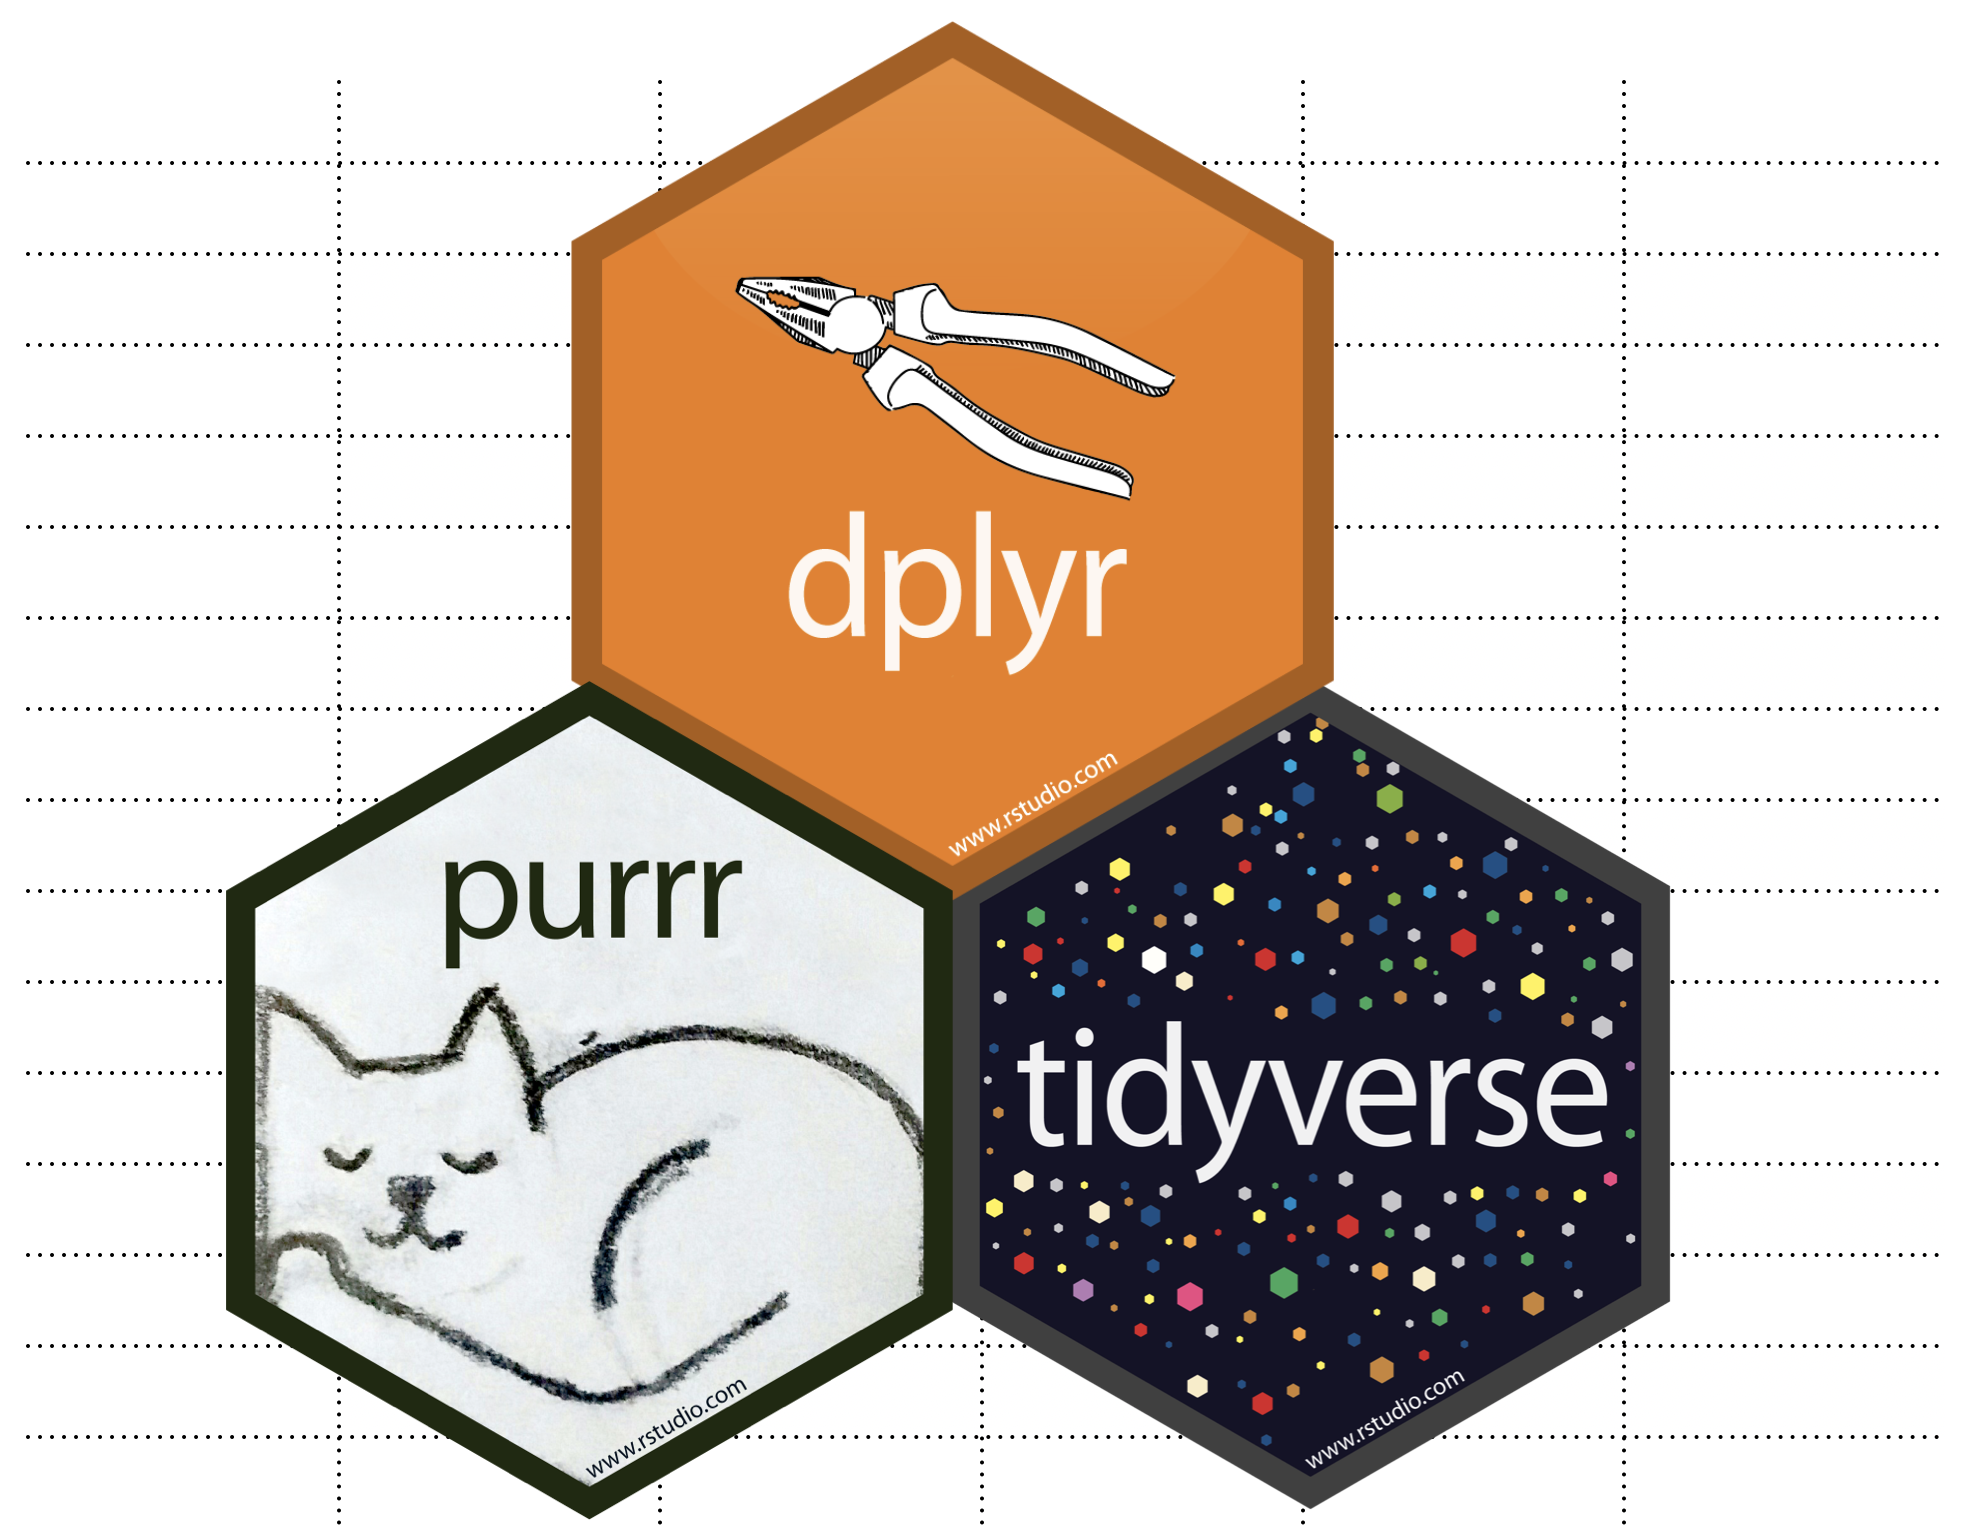
\includegraphics[width=0.7\textwidth,height=0.7\textheight]{logos/dplyrlogs.png}

}

\caption{row-wise and column-wise operations}

\end{figure}%

With the development of \textbf{dplyr} or its umbrella package
\textbf{tidyverse}, it becomes quite easy to perform operations over
columns or rows in R. These column- or row-wise methods can also be
directly integrated with other dplyr verbs like \texttt{select},
\texttt{mutate}, \texttt{filter} and \texttt{summarise}, making them
more comparable with other functions in \texttt{apply} or \texttt{map}
families. In this blog, I will briefly cover some useful column- or
row-wise operations.

\section{Column-wise operation}\label{column-wise-operation}

\textbf{Example 1:} select those string columns with less than 5 levels
in the dataset of \textbf{starwars}.

\begin{Shaded}
\begin{Highlighting}[]
\NormalTok{starwars }\SpecialCharTok{\%\textgreater{}\%}
  \FunctionTok{select\_if}\NormalTok{(}\SpecialCharTok{\textasciitilde{}} \FunctionTok{any}\NormalTok{(}\FunctionTok{is.character}\NormalTok{(.x) }\SpecialCharTok{\&} \FunctionTok{length}\NormalTok{(}\FunctionTok{unique}\NormalTok{(.x)) }\SpecialCharTok{\textless{}=} \DecValTok{5}\NormalTok{)) }\SpecialCharTok{\%\textgreater{}\%} 
  \FunctionTok{head}\NormalTok{()}
\end{Highlighting}
\end{Shaded}

\begin{verbatim}
# A tibble: 6 x 2
  sex    gender   
  <chr>  <chr>    
1 male   masculine
2 none   masculine
3 none   masculine
4 male   masculine
5 female feminine 
6 male   masculine
\end{verbatim}

We can combine \texttt{select\_if} and \texttt{any} to identify certain
columns by certain criterion. \textbf{Note:} we are using tilde
(\textasciitilde) to define an anonymous function, and thus we should
use \texttt{.x} to refer to the selected columns. See this
\href{https://www.youtube.com/watch?v=ynaHKNdAAwk&t=364s}{link} for
detailed illustration of tilde (\textasciitilde), dot (.), and dot x
(.x) in dplyr.

If you want to calculate the levels of those selected columns, you can
try \texttt{across} function and \texttt{summarise} the number of levels
by column.

\begin{Shaded}
\begin{Highlighting}[]
\NormalTok{starwars }\SpecialCharTok{\%\textgreater{}\%}
  \FunctionTok{summarise}\NormalTok{(}\FunctionTok{across}\NormalTok{(}\FunctionTok{where}\NormalTok{(is.character), }\SpecialCharTok{\textasciitilde{}} \FunctionTok{length}\NormalTok{(}\FunctionTok{unique}\NormalTok{(.x))))}
\end{Highlighting}
\end{Shaded}

\begin{verbatim}
# A tibble: 1 x 8
   name hair_color skin_color eye_color   sex gender homeworld species
  <int>      <int>      <int>     <int> <int>  <int>     <int>   <int>
1    87         12         31        15     5      3        49      38
\end{verbatim}

Alternatively, you can make use of the \texttt{map} or \texttt{map\_dbl}
function in \textbf{purrr} by the following command. Note that when a
\texttt{map} function is applied to a data.frame, it will operate over
columns by default.

\begin{Shaded}
\begin{Highlighting}[]
\CommentTok{\# map\_dbl returns a double vector, while map returns a list}
\NormalTok{starwars }\SpecialCharTok{\%\textgreater{}\%}
  \FunctionTok{select\_if}\NormalTok{(}\SpecialCharTok{\textasciitilde{}} \FunctionTok{is.character}\NormalTok{(.x)) }\SpecialCharTok{\%\textgreater{}\%}
  \FunctionTok{map\_dbl}\NormalTok{(}\SpecialCharTok{\textasciitilde{}}\FunctionTok{length}\NormalTok{(}\FunctionTok{unique}\NormalTok{(.x))) }\SpecialCharTok{\%\textgreater{}\%}
  \FunctionTok{head}\NormalTok{()}
\end{Highlighting}
\end{Shaded}

\begin{verbatim}
      name hair_color skin_color  eye_color        sex     gender 
        87         12         31         15          5          3 
\end{verbatim}

\textbf{Example 2:} select those numeric columns and calculate the means
and sds across columns in the dataset of \textbf{starwars}.

\begin{Shaded}
\begin{Highlighting}[]
\NormalTok{starwars }\SpecialCharTok{\%\textgreater{}\%}
  \FunctionTok{summarise}\NormalTok{(}\FunctionTok{across}\NormalTok{(}\FunctionTok{where}\NormalTok{(}\SpecialCharTok{\textasciitilde{}} \FunctionTok{is.numeric}\NormalTok{(.x)),}
                   \FunctionTok{list}\NormalTok{(}\AttributeTok{Mean =} \SpecialCharTok{\textasciitilde{}} \FunctionTok{mean}\NormalTok{(.x, }\AttributeTok{na.rm =} \ConstantTok{TRUE}\NormalTok{),}
                        \AttributeTok{Sd =} \SpecialCharTok{\textasciitilde{}} \FunctionTok{sd}\NormalTok{(.x, }\AttributeTok{na.rm =} \ConstantTok{TRUE}\NormalTok{))))}
\end{Highlighting}
\end{Shaded}

\begin{verbatim}
# A tibble: 1 x 6
  height_Mean height_Sd mass_Mean mass_Sd birth_year_Mean birth_year_Sd
        <dbl>     <dbl>     <dbl>   <dbl>           <dbl>         <dbl>
1        175.      34.8      97.3    169.            87.6          155.
\end{verbatim}

This example provides us a good illustration of the use of \texttt{.x}
in \textbf{dplyr} style syntax, since we have some missing values (NAs)
in certain columns. Thus, we need to specify the parameter with
\texttt{na.rm\ =\ TRUE} inside the functions.

There is indeed a more convenient and elegant way of solving this by
using the function \texttt{summarise\_if}. It allows us to select
certain columns and operate by columns like this:

\begin{Shaded}
\begin{Highlighting}[]
\NormalTok{starwars }\SpecialCharTok{\%\textgreater{}\%}
  \FunctionTok{summarise\_if}\NormalTok{(is.numeric,}
               \FunctionTok{list}\NormalTok{(}\AttributeTok{Sum =}\NormalTok{ sum, }\AttributeTok{Mean =}\NormalTok{ mean, }\AttributeTok{Sd =}\NormalTok{ sd),}
               \AttributeTok{na.rm =} \ConstantTok{TRUE}\NormalTok{)}
\end{Highlighting}
\end{Shaded}

\begin{verbatim}
# A tibble: 1 x 9
  height_Sum mass_Sum birth_year_Sum height_Mean mass_Mean birth_year_Mean height_Sd mass_Sd birth_year_Sd
       <int>    <dbl>          <dbl>       <dbl>     <dbl>           <dbl>     <dbl>   <dbl>         <dbl>
1      14143    5741.          3765.        175.      97.3            87.6      34.8    169.          155.
\end{verbatim}

\section{Row-wise operation}\label{row-wise-operation}

\textbf{Example 3:} calculate the \textbf{sums}, \textbf{means} and
\textbf{sds} for each row for the dataset of \textbf{iris}.

\begin{Shaded}
\begin{Highlighting}[]
\NormalTok{iris }\SpecialCharTok{\%\textgreater{}\%}
  \FunctionTok{rowwise}\NormalTok{() }\SpecialCharTok{\%\textgreater{}\%}
  \FunctionTok{mutate}\NormalTok{(}
    \AttributeTok{Rowsum =} \FunctionTok{sum}\NormalTok{(}\FunctionTok{c\_across}\NormalTok{(Sepal.Length}\SpecialCharTok{:}\NormalTok{Petal.Width)),}
    \AttributeTok{Rowsd =} \FunctionTok{sd}\NormalTok{(}\FunctionTok{c\_across}\NormalTok{(Sepal.Length}\SpecialCharTok{:}\NormalTok{Petal.Width)),}
    \AttributeTok{Rowmean =} \FunctionTok{mean}\NormalTok{(}\FunctionTok{c\_across}\NormalTok{(Sepal.Length}\SpecialCharTok{:}\NormalTok{Petal.Width))}
\NormalTok{  ) }\SpecialCharTok{\%\textgreater{}\%}
  \FunctionTok{ungroup}\NormalTok{() }\SpecialCharTok{\%\textgreater{}\%}
  \FunctionTok{head}\NormalTok{()}
\end{Highlighting}
\end{Shaded}

\begin{verbatim}
# A tibble: 6 x 8
  Sepal.Length Sepal.Width Petal.Length Petal.Width Species Rowsum Rowsd Rowmean
         <dbl>       <dbl>        <dbl>       <dbl> <fct>    <dbl> <dbl>   <dbl>
1          5.1         3.5          1.4         0.2 setosa    10.2  2.18    2.55
2          4.9         3            1.4         0.2 setosa     9.5  2.04    2.38
3          4.7         3.2          1.3         0.2 setosa     9.4  2.00    2.35
4          4.6         3.1          1.5         0.2 setosa     9.4  1.91    2.35
5          5           3.6          1.4         0.2 setosa    10.2  2.16    2.55
6          5.4         3.9          1.7         0.4 setosa    11.4  2.23    2.85
\end{verbatim}

Here the function \texttt{c\_across} is specifically designed to work
with \texttt{rowwise} operations. \textbf{Note:} \texttt{rowwise} groups
your data by row (class: \emph{rowwise\_df}), and it is best to
\texttt{ungroup} immediately. Of course, if you are more comfortable
with the \texttt{apply} function, you can also use the following
command:

\begin{Shaded}
\begin{Highlighting}[]
\NormalTok{iris }\SpecialCharTok{\%\textgreater{}\%}
  \FunctionTok{select}\NormalTok{(Sepal.Length}\SpecialCharTok{:}\NormalTok{Petal.Width) }\SpecialCharTok{\%\textgreater{}\%}
  \FunctionTok{apply}\NormalTok{(., }\DecValTok{1}\NormalTok{, }\ControlFlowTok{function}\NormalTok{(x) }\FunctionTok{c}\NormalTok{(}\FunctionTok{sum}\NormalTok{(x), }\FunctionTok{sd}\NormalTok{(x), }\FunctionTok{mean}\NormalTok{(x))) }\SpecialCharTok{\%\textgreater{}\%}
  \FunctionTok{as\_tibble}\NormalTok{() }\SpecialCharTok{\%\textgreater{}\%}
  \FunctionTok{t}\NormalTok{() }\SpecialCharTok{\%\textgreater{}\%}
  \FunctionTok{head}\NormalTok{()}
\end{Highlighting}
\end{Shaded}

\begin{verbatim}
   [,1]     [,2]  [,3]
V1 10.2 2.179449 2.550
V2  9.5 2.036950 2.375
V3  9.4 1.997498 2.350
V4  9.4 1.912241 2.350
V5 10.2 2.156386 2.550
V6 11.4 2.230844 2.850
\end{verbatim}

\begin{Shaded}
\begin{Highlighting}[]
\NormalTok{iris }\SpecialCharTok{\%\textgreater{}\%}
  \FunctionTok{rowwise}\NormalTok{() }\SpecialCharTok{\%\textgreater{}\%}
\NormalTok{  dplyr}\SpecialCharTok{::}\FunctionTok{mutate}\NormalTok{(}
    \AttributeTok{Rowsum =} \FunctionTok{sum}\NormalTok{(}\FunctionTok{c\_across}\NormalTok{(Sepal.Length}\SpecialCharTok{:}\NormalTok{Petal.Width)),}
    \AttributeTok{Rowmean =} \FunctionTok{mean}\NormalTok{(}\FunctionTok{c\_across}\NormalTok{(Sepal.Length}\SpecialCharTok{:}\NormalTok{Petal.Width)),}
    \AttributeTok{Rowsd =} \FunctionTok{sd}\NormalTok{(}\FunctionTok{c\_across}\NormalTok{(Sepal.Length}\SpecialCharTok{:}\NormalTok{Petal.Width)),}
    \AttributeTok{.before =} \StringTok{"Species"}
\NormalTok{  ) }\SpecialCharTok{\%\textgreater{}\%}
  \FunctionTok{ungroup}\NormalTok{() }\SpecialCharTok{\%\textgreater{}\%}
  \FunctionTok{head}\NormalTok{()}
\end{Highlighting}
\end{Shaded}

\begin{verbatim}
# A tibble: 6 x 8
  Sepal.Length Sepal.Width Petal.Length Petal.Width Rowsum Rowmean Rowsd Species
         <dbl>       <dbl>        <dbl>       <dbl>  <dbl>   <dbl> <dbl> <fct>  
1          5.1         3.5          1.4         0.2   10.2    2.55  2.18 setosa 
2          4.9         3            1.4         0.2    9.5    2.38  2.04 setosa 
3          4.7         3.2          1.3         0.2    9.4    2.35  2.00 setosa 
4          4.6         3.1          1.5         0.2    9.4    2.35  1.91 setosa 
5          5           3.6          1.4         0.2   10.2    2.55  2.16 setosa 
6          5.4         3.9          1.7         0.4   11.4    2.85  2.23 setosa 
\end{verbatim}

\begin{Shaded}
\begin{Highlighting}[]
\NormalTok{iris }\SpecialCharTok{\%\textgreater{}\%}
  \FunctionTok{as\_tibble}\NormalTok{() }\SpecialCharTok{\%\textgreater{}\%}
\NormalTok{  dplyr}\SpecialCharTok{::}\FunctionTok{mutate}\NormalTok{(}
    \AttributeTok{row =} \FunctionTok{pmap}\NormalTok{(}\FunctionTok{across}\NormalTok{(}\DecValTok{1}\SpecialCharTok{:}\DecValTok{4}\NormalTok{), }\SpecialCharTok{\textasciitilde{}}\NormalTok{ \{}
      \FunctionTok{list}\NormalTok{(}\AttributeTok{rsum =}\NormalTok{ sum, }\AttributeTok{rmean =}\NormalTok{ mean) }\SpecialCharTok{\%\textgreater{}\%}
        \FunctionTok{map\_dfc}\NormalTok{(}\ControlFlowTok{function}\NormalTok{(f) }\FunctionTok{f}\NormalTok{(}\FunctionTok{c}\NormalTok{(...)))}
\NormalTok{    \}),}
    \AttributeTok{.before =} \StringTok{"Sepal.Length"}
\NormalTok{  ) }\SpecialCharTok{\%\textgreater{}\%}
  \FunctionTok{unnest}\NormalTok{(row) }\SpecialCharTok{\%\textgreater{}\%}
  \FunctionTok{head}\NormalTok{()}
\end{Highlighting}
\end{Shaded}

\begin{verbatim}
# A tibble: 6 x 7
   rsum rmean Sepal.Length Sepal.Width Petal.Length Petal.Width Species
  <dbl> <dbl>        <dbl>       <dbl>        <dbl>       <dbl> <fct>  
1  10.2  2.55          5.1         3.5          1.4         0.2 setosa 
2   9.5  2.38          4.9         3            1.4         0.2 setosa 
3   9.4  2.35          4.7         3.2          1.3         0.2 setosa 
4   9.4  2.35          4.6         3.1          1.5         0.2 setosa 
5  10.2  2.55          5           3.6          1.4         0.2 setosa 
6  11.4  2.85          5.4         3.9          1.7         0.4 setosa 
\end{verbatim}

\begin{Shaded}
\begin{Highlighting}[]
\NormalTok{iris }\SpecialCharTok{\%\textgreater{}\%}
  \FunctionTok{as\_tibble}\NormalTok{() }\SpecialCharTok{\%\textgreater{}\%}
\NormalTok{  dplyr}\SpecialCharTok{::}\FunctionTok{mutate}\NormalTok{(}
    \AttributeTok{row =} \FunctionTok{pmap}\NormalTok{(}
      \FunctionTok{across}\NormalTok{(Sepal.Length}\SpecialCharTok{:}\NormalTok{Petal.Width),}
      \SpecialCharTok{\textasciitilde{}} \FunctionTok{bind\_cols}\NormalTok{(}
        \AttributeTok{rsum =} \FunctionTok{sum}\NormalTok{(}\FunctionTok{c}\NormalTok{(...)),}
        \AttributeTok{rmean =} \FunctionTok{mean}\NormalTok{(}\FunctionTok{c}\NormalTok{(...)),}
        \AttributeTok{rsd =} \FunctionTok{sd}\NormalTok{(}\FunctionTok{c}\NormalTok{(...))}
\NormalTok{      )}
\NormalTok{    ),}
    \AttributeTok{.before =} \StringTok{"Sepal.Length"}
\NormalTok{  ) }\SpecialCharTok{\%\textgreater{}\%}
  \FunctionTok{unnest}\NormalTok{(row) }\SpecialCharTok{\%\textgreater{}\%}
  \FunctionTok{head}\NormalTok{()}
\end{Highlighting}
\end{Shaded}

\begin{verbatim}
# A tibble: 6 x 8
   rsum rmean   rsd Sepal.Length Sepal.Width Petal.Length Petal.Width Species
  <dbl> <dbl> <dbl>        <dbl>       <dbl>        <dbl>       <dbl> <fct>  
1  10.2  2.55  2.18          5.1         3.5          1.4         0.2 setosa 
2   9.5  2.38  2.04          4.9         3            1.4         0.2 setosa 
3   9.4  2.35  2.00          4.7         3.2          1.3         0.2 setosa 
4   9.4  2.35  1.91          4.6         3.1          1.5         0.2 setosa 
5  10.2  2.55  2.16          5           3.6          1.4         0.2 setosa 
6  11.4  2.85  2.23          5.4         3.9          1.7         0.4 setosa 
\end{verbatim}

\section{Related links:}\label{related-links}

\begin{itemize}
\tightlist
\item
  \url{https://dplyr.tidyverse.org/articles/rowwise.html}
\item
  \url{https://purrr.tidyverse.org/reference/map.html}
\end{itemize}




\end{document}
